\section{\textit{Coverage}}
  
  Usualmente, cuando estamos escribiendo tests, nos gustaría saber qué funcionalidades estamos
  probando.
  El \textit{coverage} es una métrica que nos permite saber qué porcentaje de nuestro código
  está siendo probado por los tests.

  \begin{important}
    Tener un buen \textit{coverage} no es garantía de que nuestro código esté bien testeado, es sólo
    una métrica que nos permite saber qué porcentaje de nuestro código está siendo probado.
  \end{important}

  \textit{Kotest} provee de una herramienta para medir el \textit{coverage} de nuestros tests.
  Para utilizarlo, debemos dar click derecho sobre la carpeta \url{src/test/kotlin} y seleccionar
  `\textit{More Run/Debug}' y luego `\textit{Run `Tests in `kygo.test'' with Coverage}' 
  (\cref{fig:coverage}).

  \begin{figure}[ht!]
    \centering
    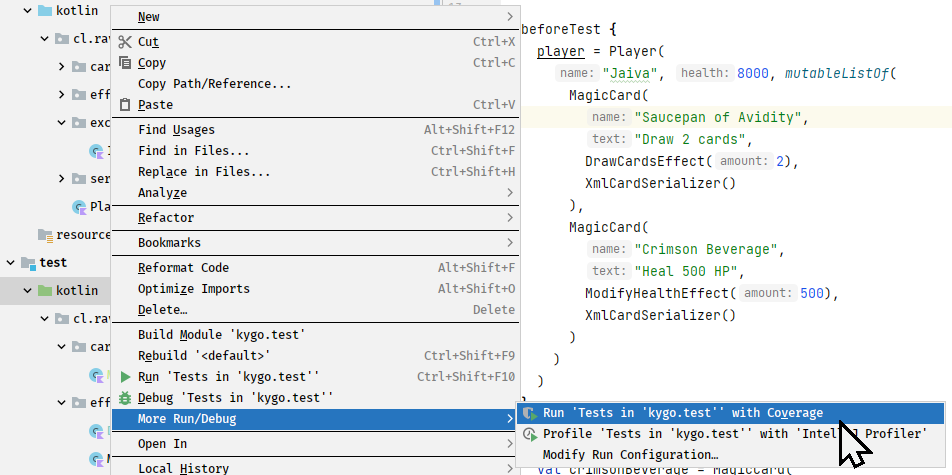
\includegraphics[width=0.8\textwidth]{img/oop/strategy/run_with_coverage.png}
    \caption{Correr tests con \textit{coverage}}
    \label{fig:coverage}
  \end{figure}

  Una vez que los tests terminen de correr, se abrirá una ventana con el \textit{coverage} de los
  tests (\cref{fig:coverage:report}).
  Aquí veremos cuatro columnas:

  \begin{itemize}
    \item \textbf{\textit{Element}:} Nombre del paquete o clase que se está probando.
    \item \textbf{\textit{Class}:} Porcentaje de las clases que se están probando.
    \item \textbf{\textit{Method}:} Porcentaje de los métodos que se están probando.
    \item \textbf{\textit{Line}:} Porcentaje de las líneas que se están probando.
  \end{itemize}

  \begin{figure}[ht!]
    \centering
    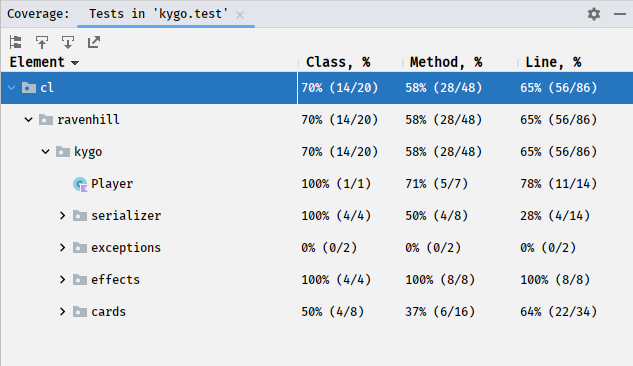
\includegraphics[width=0.8\textwidth]{img/oop/strategy/coverage_report.png}
    \caption{Reporte de \textit{coverage}}
    \label{fig:coverage:report}
  \end{figure}

  En general, se recomienda tener un \textit{coverage} de al menos 90\% de las líneas.
  Para saber qué lineas están siendo probadas, \textit{Kotest} marcará con un color verde las líneas
  que están siendo probadas y con un color rojo las líneas que no están siendo probadas como se
  muestra en la \cref{fig:coverage:report:lines}.

  \begin{figure}[ht!]
    \centering
    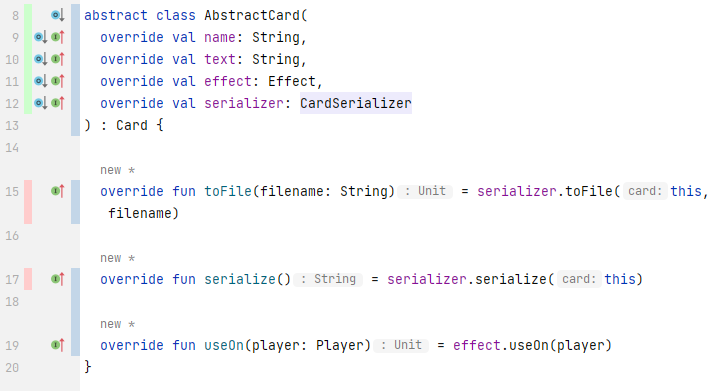
\includegraphics[width=0.8\textwidth]{img/oop/strategy/coverage_report_lines.png}
    \caption{
      A la izquierda se marca con un color verde las líneas que están siendo probadas y con un color
      rojo las líneas que no están siendo probadas.
    }
    \label{fig:coverage:report:lines}
  \end{figure}

  Notarán que las líneas que están marcadas con rojo son las de los métodos 
  \mintinline{kotlin}|toFile(String)| y \mintinline{kotlin}|serialize| de la clase
  \mintinline{kotlin}|AbstractCard|.
  
  Escribamos los tests para estos métodos.
  Noten que como no podemos instanciar una clase abstracta, vamos a tener que probar el método en
  sus subclases.
  Como los métodos están definidos en la clase abstracta, sabemos que hacen lo mismo en todas las
  subclases, así que podemos crear un \textit{test factory} para reusar el código de los tests.

  \begin{kotlin}
    fun `a card can be serialized to a string`(card: Card, serializedString: String) =
      funSpec {
        test("a card can be serialized to a string") {
          card.serialize() shouldBe serializedString
        }
      }
  \end{kotlin}

  \begin{kotlin}
    fun `a card can be serialized to a file`(
      card: Card, filename: String, serializedString: String
    ) = funSpec {
      lateinit var file: File

      beforeTest {
        file = File(filename)
      }

      afterTest {
        file.delete()
      }

      test("a card can be serialized to a file") {
        card.toFile(filename)
        file.readText() shouldBe serializedString
      }
    }
  \end{kotlin}

  Aquí tenemos algo nuevo, la función \mintinline{kotlin}|afterTest|.
  Esta función es similar a la función \mintinline{kotlin}|beforeTest|, pero se ejecuta después de
  cada test.
  En general se usa para \enquote{limpiar} el estado del sistema después de cada test.
  En este caso, estamos borrando el archivo que creamos para el test.

  Ahora podemos crear los tests para las clases que concretizan a \texttt{Card}:

  \begin{kotlin}
    class MagicCardTest : FunSpec({
      ...
      include(`a card can be serialized to a string`(
        MagicCard(
          "Saucepan of Avidity",
          "Draw 2 cards",
          DrawCardsEffect(2),
          XmlCardSerializer()
        ),
        """
          |<Card>
          | <name>Saucepan of Avidity</name>
          | <text>Draw 2 cards</text>
          |</Card>
          """.trimMargin()
      ))
      include(`a card can be serialized to a file`(
        MagicCard(
          "Saucepan of Avidity",
          "Draw 2 cards",
          DrawCardsEffect(2),
          XmlCardSerializer()
        ),
        "saucepan_of_avidity.xml",
        """
          |<Card>
          | <name>Saucepan of Avidity</name>
          | <text>Draw 2 cards</text>
          |</Card>
          """.trimMargin()
      ))
    })
  \end{kotlin}